\section{Diskussion}
\label{sec:Diskussion}
In \autoref{tab:fazit} sind die Elementarladung in unkorrigierter und korrigierter Form und die Avogadrokonstante
angegeben. Weiterhin sind noch die entsprechenden Literaturwerte und deren Abweichungen gegeben. Der Literaturwert
für die Elementarladung beträgt $e=1,602\cdot 10^{-19}$ \cite{e} und der der Avogadrokonstante $N_{\symup{A}}=
6,022\cdot 10^{23}$ \cite{avogadro}.

\begin{table}
    \centering
    \caption{Experimentell bestimmte Größen, deren Literaturwerte und Abweichungen zum Literaturwert.}
    \label{tab:fazit}
    \begin{tabular}{c | c c c}
        \toprule
        Größe & Experimentell & Literaturwert & Relative Abweichung \\
        \midrule
        $e_{\symup{0}}$         & $(1,1 \pm 1,4)\cdot 10^{-19}\,\si{\coulomb}$  & $1,602\cdot 10^{-19}\,\si{\coulomb}$  & $45,64\,\%$ \\
        $e_{\symup{0, korr}}$   & $(1,3 \pm 1,2)\cdot 10^{-19}\,\si{\coulomb}$  & $1,602\cdot 10^{-19}\,\si{\coulomb}$  & $23,23\,\%$ \\
        $N_{\symup{A}}$         & $(8 \pm 7)\cdot 10^{23}\,\frac{1}{\si{\mol}}$ & $6,022\cdot 10^{23}$                  & $32,85\,\%$ \\ 
        \bottomrule
    \end{tabular}
\end{table}

\addsec{Anhang}
\label{sec:Anhang}

\begin{figure}
    \centering
    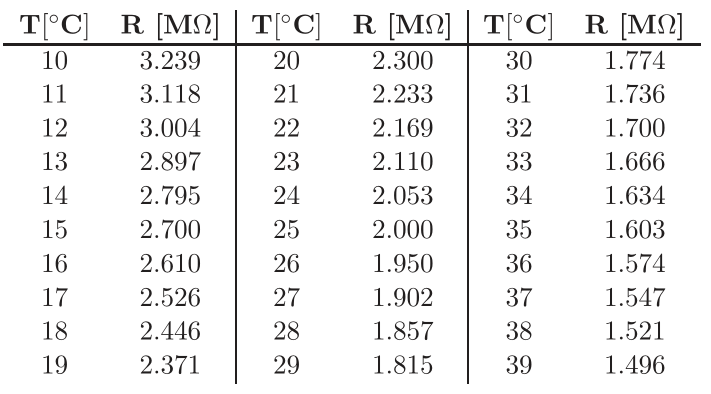
\includegraphics[width=0.7\textwidth]{bilder/thermistorwiderstand.png}
    \caption{Thermistor-Widerstandstabelle \cite{sample}.}
    \label{fig:thermistor}
\end{figure}

\begin{figure}
    \centering
    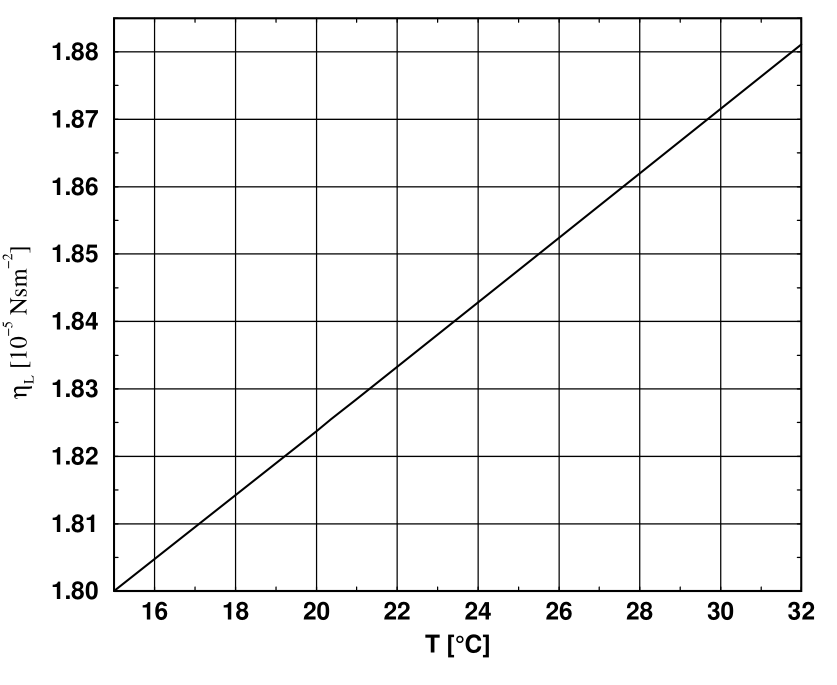
\includegraphics[width=0.7\textwidth]{bilder/viskositaet.png}
    \caption{Viskosität der Luft in Abhängigkeit der Temperatur \cite{sample}.}
    \label{fig:viskositaet}
\end{figure}

\begin{figure}
    \centering
    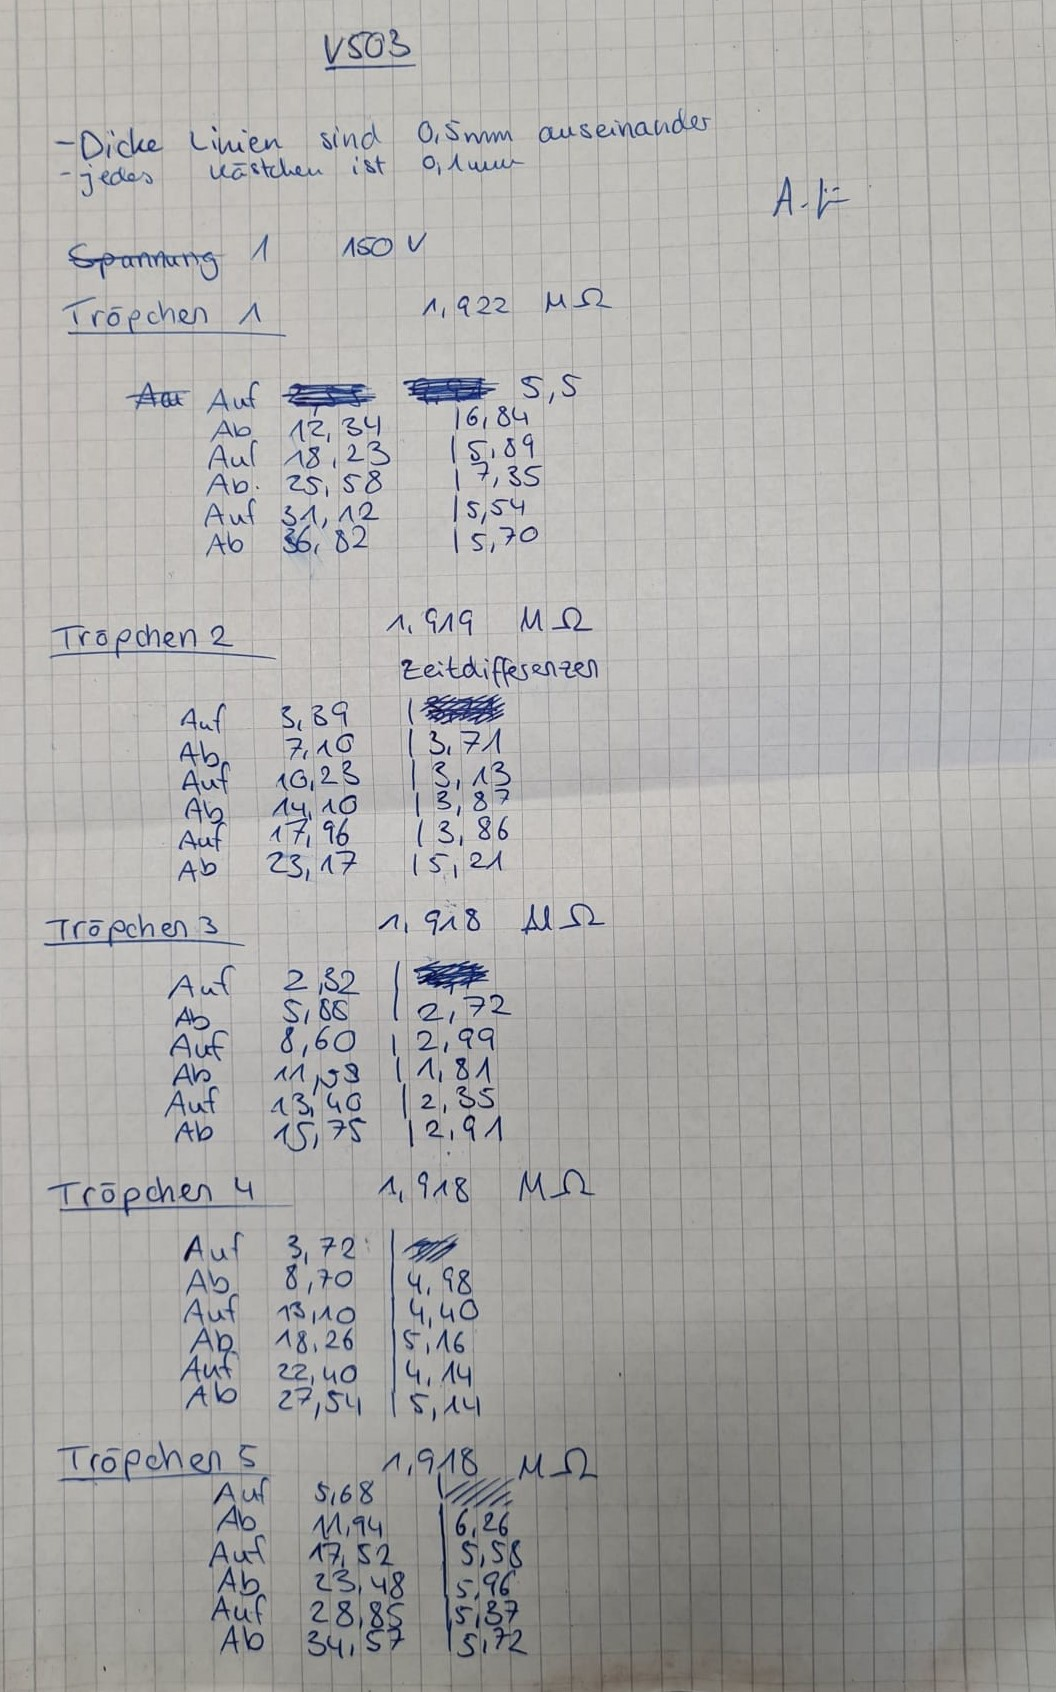
\includegraphics[width=0.7\textwidth]{bilder/Spannung1.jpg}
    \caption{Messwerte der ersten Spannung.}
\end{figure}

\begin{figure}
    \centering
    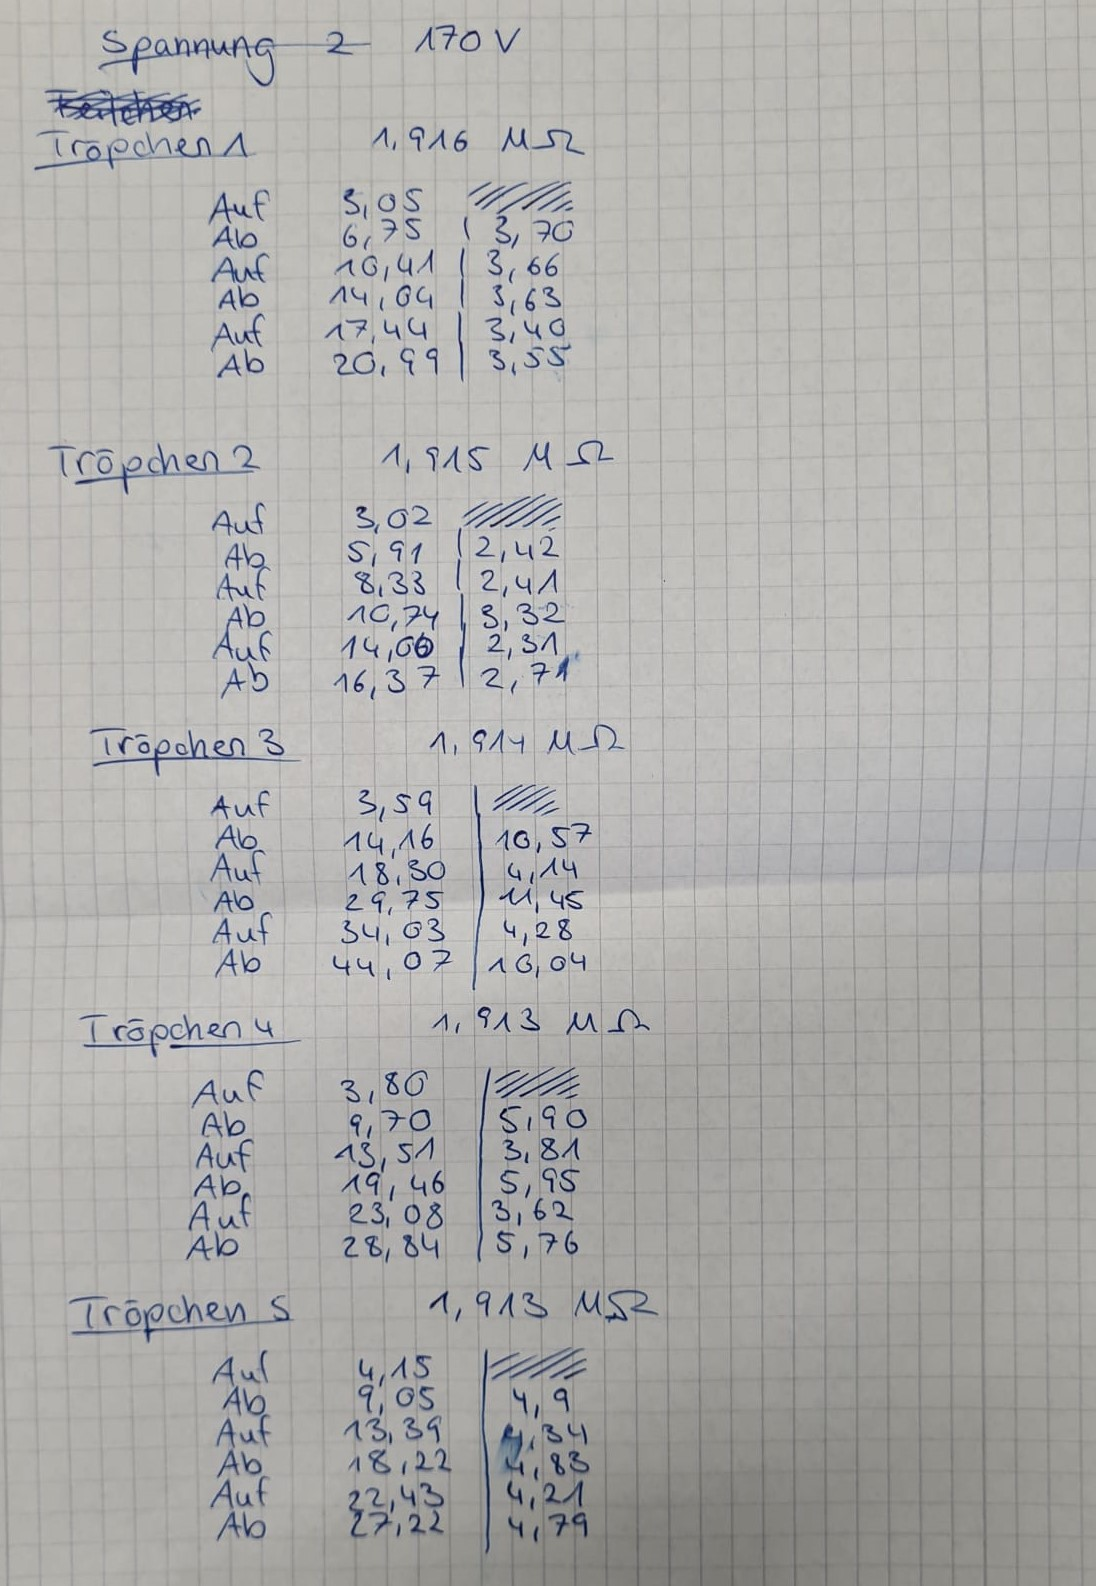
\includegraphics[width=0.7\textwidth]{bilder/Spannung2.jpg}
    \caption{Messwerte der zweiten Spannung.}
\end{figure}

\begin{figure}
    \centering
    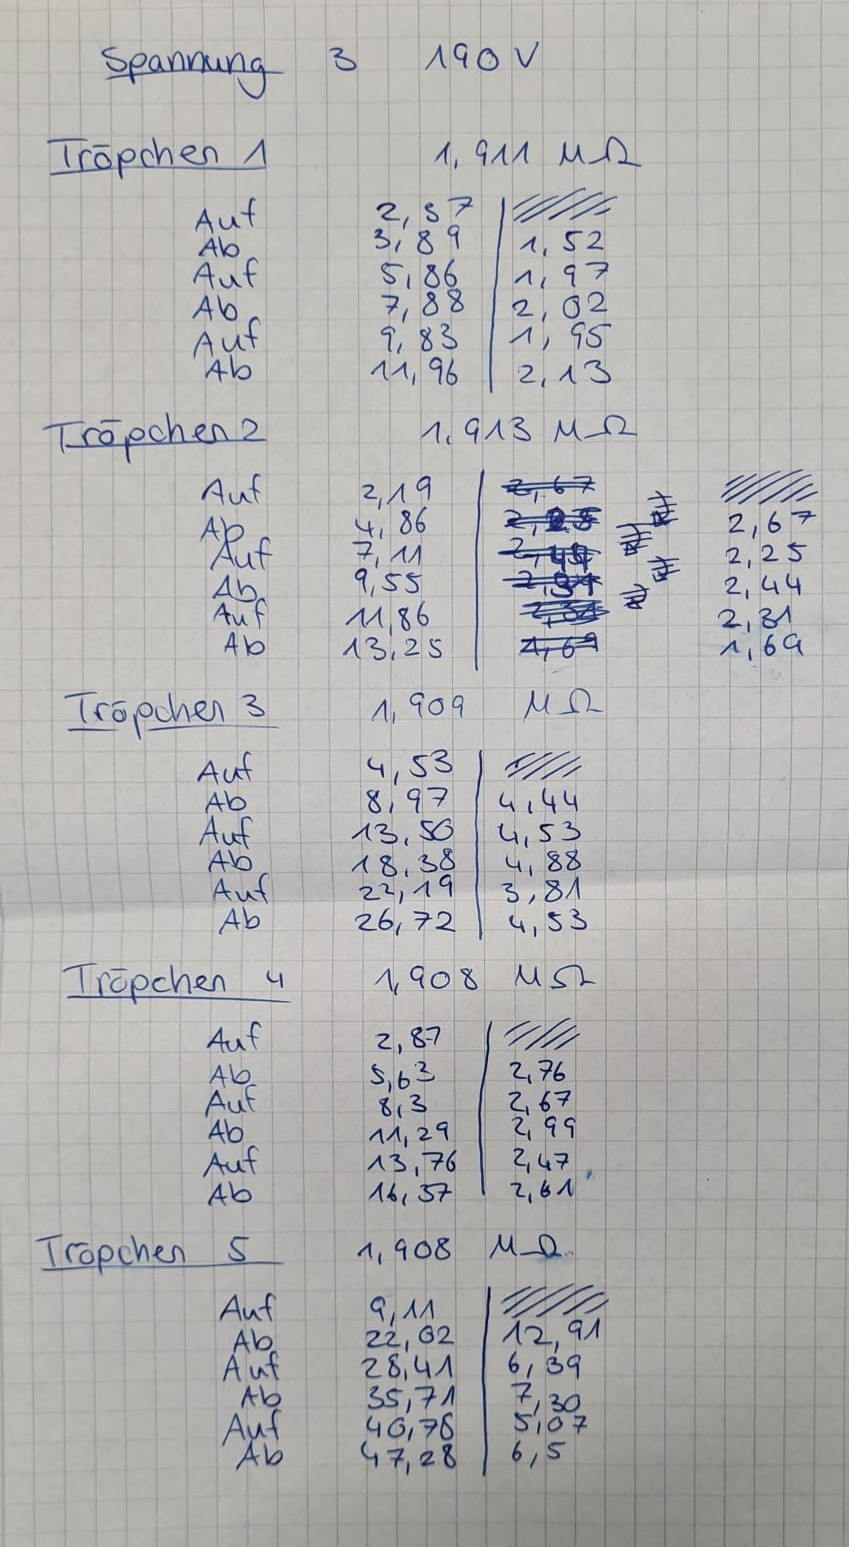
\includegraphics[width=0.7\textwidth]{bilder/Spannung3.jpg}
    \caption{Messwerte der dritten Spannung.}
\end{figure}

\begin{figure}
    \centering
    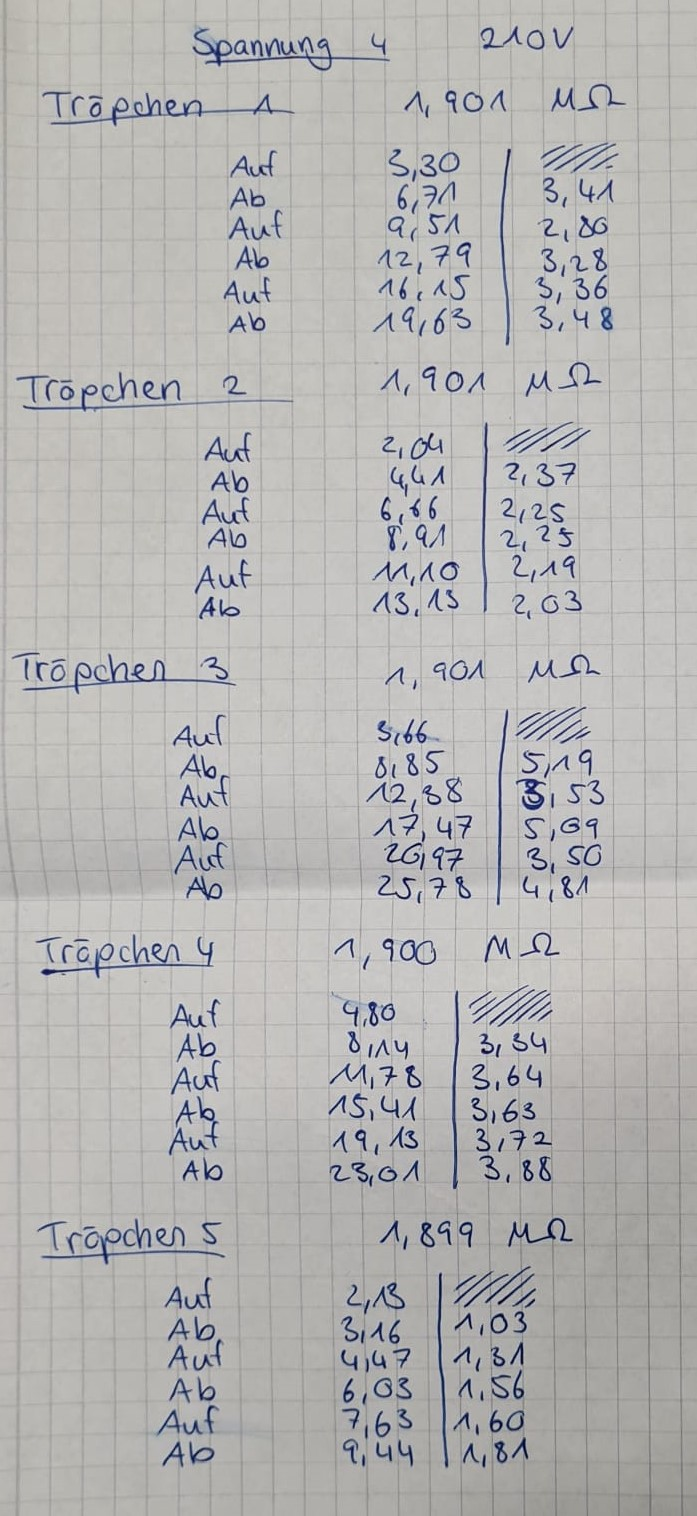
\includegraphics[width=0.7\textwidth]{bilder/Spannung4.jpg}
    \caption{Messwerte der vierten Spannung.}
\end{figure}

\begin{figure}
    \centering
    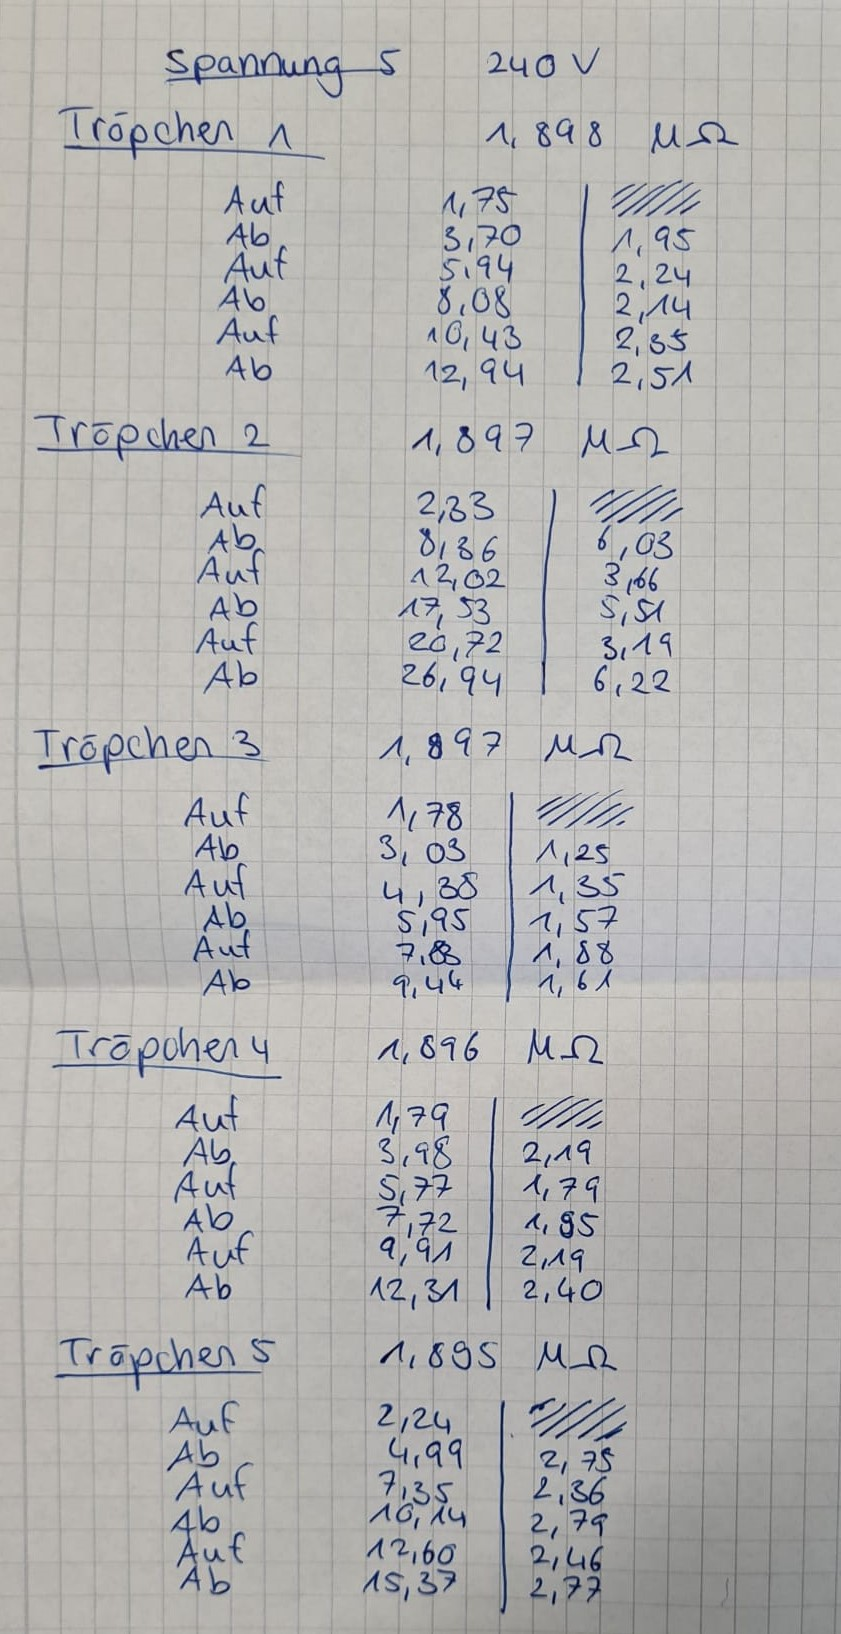
\includegraphics[width=0.7\textwidth]{bilder/Spannung5.jpg}
    \caption{Messwerte der fünften Spannung.}
\end{figure}